\section{Data gathering}

From here, the procedure and the environment of gathering information to elaborate approaches will be discussed in detail.

\subsection{Test environment}

In order to find scan ranges that are likely to be answered positively, data from as many ECUs as possible is needed. In the context of the PetS3 project a remote testing environment has been created. This was particularly helpful in light of the contact limitations at the time of writing.

The infrastructure of Laboratory for Safe and Secure Systems (LaS3) was used for that. Specifically, their GitLab server was used, displayed in \autoref{fig:gitlab-screenshot}.

%GitLab screenshot
\begin{figure}[h]
    \centering
    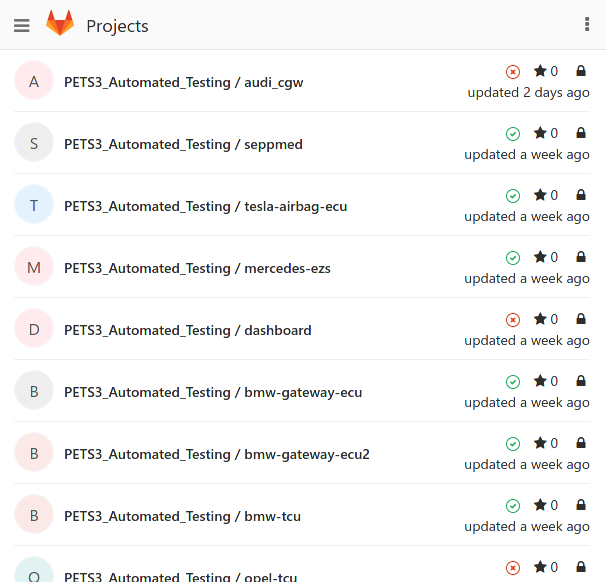
\includegraphics[width=0.7\textwidth]{gitlab-screenshot}
    \caption{Screenshot of the GitLab server.}
    \label{fig:gitlab-screenshot}
\end{figure}

Fourteen ECUs are available for testing on this server. Three of them are from Opel and thus only support GMLAN but not UDS.

For each ECU a YAML configuration file has been created. Various work is done here, for example installing this CAN-ISOTP module, if the running device is not at least on Linux 5.10 (see \autoref{sec:scapy}). Also, the current Scapy tree from the currently working branch is pulled and checked out.

Then, the actual tests are executed that are written in the pytest framework. Here, a UDS scan can be started. At the same time, another process is started to record all CAN traffic that takes place during the execution of the tests.

Finally, the resulting files are uploaded to the GitLab server so that they can be downloaded via a browser program.

\subsection{Explaining the stored data from one scan}

In total, five files are stored after a scan, which will be explained in this section.

\begin{itemize}
    \item candump.log
    \item generic.log
    \item profiling.csv
    \item milestones.csv
    \item data.pkl
\end{itemize}

\subsection{Profiling the UDS Scanner}
